\phantomsection
\addcontentsline{toc}{chapter}{Preface: Digital Communication -- A Future Technology}
\chapter*{Preface: Digital Communication -- A Future Technology}

\begin{refsection}

The current time during the Corona lockdown shows the great significance of telecommunication. It is self-evident to have access to online media and communication platforms. The internet helps to keep in touch with our loved ones. A huge amount of entertainment relies on internet access. The internet is highly integrated in our every-day life. Furthermore, it is a growing economy. There are not only the online services like social media or online warehouses which are going to expand their business in the future. The communication technologies, which the internet is built upon, are a growing and innovative market, too. Besides consumers, the \ac{B2B} market is a huge driver of innovation. It must be expected, that more devices get interconnected. This is a challenge because physical resources are limited. Nevertheless, it is a great possibility for the communication technology to advance. The technologies, which are able to cope with the new requirementes, are digital. This where the course on \emph{Digital Communication Systems} starts. You are warmly welcomed!

\addcontentsline{toc}{section}{History of Communications}
\section*{History of Communications}

Let's go back to the roots! Communication is the most important property of human beings. The spoken language has always been the most important instrument of communication between human.

An early innovation in communication technology is the written language. Information can now be conserved for a long time and even be transferred to other places. Modern societies would not be possible without written language.

Transferring information became more important as societies advanced.
\begin{itemize}
	\item People all over the world used drums or other devices to generate sounds.
	\item Some Native Americans tribes used smoke signs to communicate over large distances.
	\item The invention of paper simplified communication. Large amount of information could be stored and transferred.
	\item An example of more sophisticated communication technology is the \index{Caesar cipher} Caesar cipher used in the Roman Empire in ancient times. It is one of the first devices developed for cryptography.
	\item Homing pigeons delivered letters over long distances.
	\item In the Middle Ages, beacons were used in defensive communication to relay a signal.
	\item In the 18th century, semaphore lines had been built. They used visual telegraphy. Semaphores on fixed towers could display a set of symbols, which were relayed along the line.
\end{itemize}

\begin{minipage}{0.45\linewidth}
	\begin{figure}[H]
		\centering
		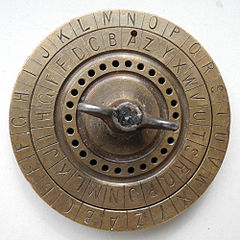
\includegraphics[width=\linewidth]{../chapter00/CaesarCipher.jpg}
		\caption[Caesar cipher]{Caesar cipher. Each letter is replaced by another one which is a fixed number of letters away from the original one. \licensequote{\cite{Berberich2013}}{Hubert Berberich}{Public Domain}}
	\end{figure}
\end{minipage}
\hfill
\begin{minipage}{0.45\linewidth}
	\begin{figure}[H]
		\centering
		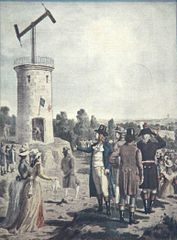
\includegraphics[width=\linewidth]{../chapter00/OpticalTelegraph.jpg}
		\caption[Optical telegraph]{Optical telegraph \cite{WikiSemaphore}}
	\end{figure}
\end{minipage}

The research of electricity created the foundations for modern communication systems. Electrical telegraphy speeded up telecommunication. At the end of the 19th century, electromagnetic waves have been discovered. James Clerk Maxwell postulated them in 1865. Heinrich Hertz produced the first electromagnetic waves in 1887. The potential had soon been acknowledged by inventors, who developed first radios. The era of analogue radio communication began. The \index{vacuum tube} vacuum tube became an important component in radio electronics.

In 1947, the bipolar transistor had been invented. This marked the beginning of the semiconductor era, which still endures. Over the decades, semiconductors became more integrated. In 1958, the first \ac{IC} had been demonstrated by Jack Kilby, engineer at Texas Instruments. At this time, wireless communication was mostly restricted to broadcasting and professional users.

With the 1990s, wireless communication technologies became more and more affordable for private usage. Advancing computer since was incorporated into communication systems. Digital communication systems gained significance and started superseding analogue communication technologies.

\addcontentsline{toc}{section}{An Innovation Motor}
\section*{An Innovation Motor}

Nowadays, innovations are driven by the demand for telecommunication which especially
\begin{itemize}
	\item is fast,
	\item is reliable,
	\item is secure,
	\item has higher throughput, and
	\item reduces the cost.
\end{itemize}

Speed and data rate are important measures, which are advertised by companies selling their products. For example, the entertainment industry like video-on-demand services require more bandwidth to deliver video streams of higher quality. Stock exchanges need low latency to trade securities within milliseconds.

Reliability is a key requirement for critical infrastructure. An unreliable system may result in loss of production or may even lead to serious dangers for health and life of people. For example, railroad traffic management requires extremely reliable communication systems for high-speed trains to prevent accidents. This goes along with security. Unauthorized parties shall have no access to the communication system. Data integrity and privacy are important.

There is often a trade-off between different requirements. No technology can fit all requirements equally. The greatest challenge for an engineer, working on Digital Communications Systems, is finding the optimal solution, which fits the customer's wishes best.

As a general rule, cost reduction is the main argument for businesses to adapt new technologies. Other requirements must of course fit. However, technologies are unlike to be implemented if they increase the monetary costs for the user.


\addcontentsline{toc}{section}{Unlimited Possibilities}
\section*{Unlimited Possibilities}

Each interconnected electronic component is a communication system. Even if a device does not communicate with its environment, its interconnected components may exchange data with each other. This shows the significance of digital communication systems. In addition, many devices provide a digital communication interface or radio link to interconnect with other devices.

Understanding digital communication systems is of great importance in many engineering and non-engineering fields, for example:
\begin{itemize}
	\item \textbf{Automation} -- The components of an automation system are interconnected. There are bus systems like ProfiBus in machine control. Non-safety applications may use wireless systems (RFID in logistics, etc.).
	\item \textbf{Medical Systems} -- Telemedicine requires broadband systems for communication between health care professionals or between a health care professional and a patient. Robotic surgery has tight requirements on latency and reliability.
	\item \textbf{Transport} -- Public infrastructure (railway, air traffic) need safety systems. Aeronautical radio is the basis for air traffic management. Vehicles like high-speed trains, aircrafts or cars require communication devices on board so that their components can 
	\item \textbf{Public Safety} -- Authorities and organizations responsible for safety (police, fire brigades, civil protection) must reliably exchange information to run their missions.
	\item \textbf{Agriculture} -- Future agriculture uses sensors to observe soil parameters, vital signs of animals, etc. Weather forecasts would be impossible without communication technology (weather radar, weather satellites).
	\item \textbf{Energy Sector} -- Smart grids rely on information exchange between energy producers and energy consumers. Communication technologies enable an efficient control of the power network.
\end{itemize}

\printbibliography[heading=subbibliography]
\end{refsection}
